\subsection{In-Context Learning}
\label{subsec-icl}
As a special prompting form, in-context learning~(ICL) is first proposed along with GPT-3~\cite{Brown-NeurIPS-2020-Language}, which has become a typical approach to utilizing LLMs. 

\subsubsection{ICL Formulation}
\label{subsubsec-icl-formulation}

As stated in~\cite{Brown-NeurIPS-2020-Language}, ICL uses a formatted natural language prompt, consisting of the task description and/or a few task examples as demonstrations.
Figure~\ref{fig:utilization} presents an illustration of ICL.
First, starting with a task description, a few examples are selected from the task dataset as demonstrations.
Then, they are combined in a specific order to form natural language prompts with specially designed templates.
Finally, the test instance is appended to the demonstration as the input for LLMs to generate the output.
Based on task demonstrations, LLMs can recognize and perform a new task without explicit gradient update.

Formally, let $D_k = \{ f(x_1, y_1), \dots, f(x_k, y_k) \}$ represent a set of demonstrations with $k$ examples, where $f(x_k, y_k)$ is the prompt function that transforms the $k$-th task example into natural language prompts.
Given the task description $I$, demonstration $D_k$, and a new input query $x_{k+1}$, the prediction of the output $\hat{y}_{k+1}$ generated from LLMs can be formulated as follows\footnote{
When ICL was introduced in the GPT-3's paper~\cite{Brown-NeurIPS-2020-Language}, it was originally defined to be a combination of the task description and demonstration examples, wherein either component is dispensable. Following this definition, when a LLM is required to solve an unseen task by using only task descriptions, it can be also considered to perform ICL for task solving, whereas the ICL ability can be enhanced by instruction tuning.   
}: 
\begin{equation}\label{eq-ICL-prompting}
     \text{LLM} \big(I, \underbrace{ f(x_1, y_1), \dots, f(x_k, y_k)}_{\text{demonstrations}}, f(\underbrace{x_{k+1}}_{\text{input}}, \underbrace{\vphantom{\hat{y}_{k+1}} \_\_\_}_{\text{answer}}) \big) \rightarrow \hat{y}_{k+1}.
\end{equation}
where the actual answer $y_{k+1}$ is left as a blank to be predicted by the  LLM. %
Since the performance of ICL heavily relies on demonstrations, it is important to properly design them in the prompts. 
According to the construction process in Equation~\eqref{eq-ICL-prompting}, we focus on three major aspects of formatting demonstrations in the prompts, including how to select examples that make up demonstrations, format each example into the prompt with the function $f(\cdot)$, and arrange demonstrations in a reasonable order.  

{
A comprehensive review of ICL has been presented in the survey paper~\cite{Dong-arxiv-2023-A}, and we suggest the readers referring to it for a more general, detailed discussion on this topic. Compared with this survey, we specially focus on the discussion of applying ICL to LLMs in two major aspects, \ie demonstration design and the underlying mechanism of ICL. 
}
Also, ICL has a close connection with instruction tuning (discussed in Section~\ref{sec-instruction}) in that  
{both utilize natural language to format the task or instances}. 
However, instruction tuning needs to fine-tune LLMs for adaptation, while ICL only prompts LLMs for utilization.  
{Furthermore, instruction tuning can enhance the ICL ability of LLMs to perform target tasks, especially in the zero-shot setting (only using task descriptions)~\cite{Chung-arxiv-2022-Scaling}.  
}

\begin{figure*}[t]
    \centering
    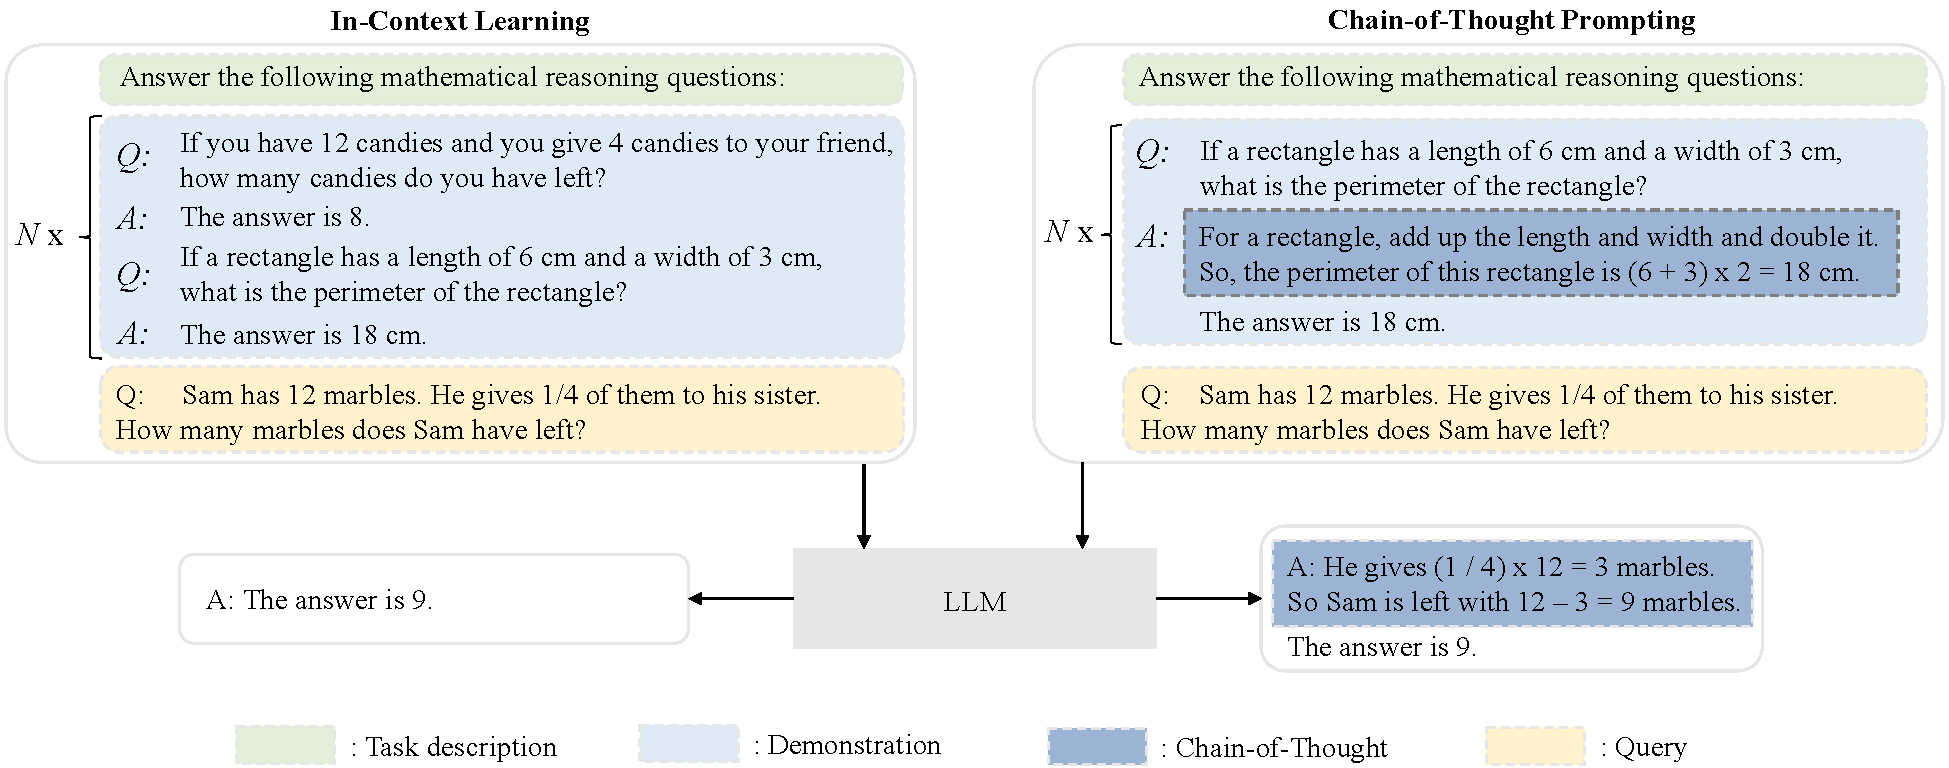
\includegraphics[width=\textwidth]{images/utilization.pdf}
    \caption{
        A comparative illustration of in-context learning~(ICL) and chain-of-thought~(CoT) prompting. 
        ICL prompts LLMs with a natural language description, several demonstrations, and a test query, while  
        CoT prompting involves a series of intermediate reasoning steps in prompts.
    }
    \label{fig:utilization}
\end{figure*}

\subsubsection{Demonstration Design}
{Several studies have shown that the effectiveness of ICL is highly affected by the design of demonstrations~\cite{Min-EMNLP-2022-Rethinking, Lu-ACL-2022-Fantasically,Zhao-ICML-2021-Calibrate}}
Following the discussion in {Section~\ref{subsubsec-icl-formulation}}, we will introduce the demonstration design of ICL from three major aspects, \ie demonstration selection, format, and order.

\paratitle{Demonstration Selection.}
{
The performance of ICL tends to have a large variance with different demonstration examples~\cite{Liu-ACL-2022-What}, so it is important to select a subset of examples that can effectively leverage the ICL capability of LLMs.}
There are two main demonstration selection approaches, namely heuristic and LLM-based approaches:


$\bullet$~\emph{Heuristic approaches.}  
{Due to their simplicity and low costs,} existing work widely adopts heuristic methods to select demonstrations.
Several studies employ a $k$-NN based retriever to select examples that are semantically relevant to the query~\cite{Liu-ACL-2022-What, Lee-COLING-2022-Does}.
{However, they perform the selection individually for each example, rather than evaluating the example set as a whole.}
To resolve this issue, diversity-based selection strategies are proposed to choose the most representative set of examples for specific tasks~\cite{Levy-arxiv-2022-Diverse, Su-arxiv-2022-selective}.
Furthermore, in~\cite{Ye-arxiv-2022-Complementary}, both relevance and diversity are taken into consideration when selecting demonstrations.


$\bullet$~\emph{LLM-based approaches.}  
Another line of work selects demonstrations by making use of LLMs. 
For example, LLMs can be utilized to directly measure the informativeness of each example according to the performance gain after adding the example~\cite{Li-arxiv-2023-Finding}. 
In addition, EPR~\cite{Rubin-NAACL-2022-Learning} proposes a two-stage retrieval approach that first recalls similar examples with an unsupervised method (\eg BM25) and then ranks them using a dense retriever (trained with positive and negative examples labeled by LLMs).
As an alternative approach, the task of demonstration selection can be formulated into a RL problem, where LLMs serve as the reward function to provide feedback for training the policy model~\cite{Zhang-EMNLP-2022-Active}. Since LLMs perform well for text annotation~\cite{Gilardi-arXiv-2023-Crowd}, some recent studies employ LLM itself as the demonstration generator without human intervention~\cite{Kim-arxiv-2022-Self-Generated}. 

{To summarize, as discussed in~\cite{Michael-ICLR-2022-An}, the selected demonstration examples in ICL should contain sufficient information about the task to solve as well as be relevant to the test query, for the above two selection approaches.} 

\paratitle{Demonstration Format.}
After selecting task examples, the next step is to integrate and format them into a natural language prompt for LLMs. 
A straightforward method is to instantiate a pre-defined template with the corresponding input-output pairs~\cite{Liu-survey-2023-Pre-train}.
To construct more informative templates, recent studies consider adding task descriptions~\cite{Chung-arxiv-2022-Scaling} or enhancing the reasoning capability of LLMs with chain-of-thought prompts~\cite{Wei-arxiv-2022-chain}.
For instance, in~\cite{Mishra-ACL-2022-Cross}, the authors collect a large-scale dataset with task descriptions written by humans.
After tuning with this dataset, the performance on seen tasks can be boosted, and LLMs can also generalize to unseen tasks to some extent.
To reduce the annotation costs, a semi-automated approach has been proposed in~\cite{Wang-arXiv-2022-Self} by employing a seed set consisting of human-written task descriptions to guide LLMs to generate task descriptions for new tasks. 
Since it is costly to manually annotate demonstration formats for different tasks, some work also studies how to automatically generate high-quality ones. 
As two representative methods, Auto-CoT~\cite{Zhang-arxiv-2022-Automatic} leverages LLMs with the zero-shot prompt ``\emph{Let’s think step by step}'' for generating intermediate reasoning steps, while least-to-most prompting~\cite{Zhou-arxiv-2022-Least} first queries LLMs to perform problem decomposition and then utilizes LLMs to sequentially solve sub-problems based on the intermediate answers to previously solved ones.  

\paratitle{Demonstration Order.}
LLMs are shown to sometimes suffer from the {recency} bias, \ie they are prone to repeat answers that are near the end of demonstrations~\cite{Zhao-ICML-2021-Calibrate}. 
Thus, it is important to arrange demonstrations (\ie task examples) in a reasonable order.
Early work proposes several heuristic methods to quickly find a good order.  
For example, demonstrations can be directly organized according to their similarity to the query in the embedding space~\cite{Liu-ACL-2022-What}: the more similar, the closer to the end.
In addition, global and local entropy metrics can be used to score different demonstration orders~\cite{Lu-ACL-2022-Fantasically}. 
To integrate more task information, some recent studies propose to minimize the  
{code length} required to compress and transmit task labels, which is inspired by information theory~\cite{Wu-arxiv-2022-Self}.
However, these methods need additional labeled data as the {validation set to evaluate the performance of specific demonstration orders}. 
To eliminate this need, the authors in~\cite{Lu-ACL-2022-Fantasically} propose to sample the validation data from the LLM itself. 

\subsubsection{Underlying Mechanism}
\label{sec-ICL-mechanism}
After pre-training, LLMs can exhibit intriguing ICL capability without being updated.  
In what follows, we discuss two key questions about the ICL ability of LLMs, \ie ``\emph{how does pre-training affect the ICL ability}'' and ``\emph{how do LLMs perform ICL during inference}''.

\paratitle{How Pre-Training Affects ICL?} 
ICL is first proposed in GPT-3~\cite{Brown-NeurIPS-2020-Language}, and it has been shown that the ICL ability becomes more significant with a larger model size.
Further, some studies reveal that small-scale PLMs can also demonstrate a strong ICL ability by continual pre-training~\cite{Gu-arXiv-2023-Pre} or fine-tuning~\cite{Min-NAACL-2022-MetaICL} on specially designed training tasks, which typically involve additional task examples in the input during the training process.
It suggests that the design of training tasks is an important influence factor on the ICL capability of LLMs. 
Besides training tasks, recent studies have also investigated the relationship between ICL and pre-training corpora~\cite{Michael-ICLR-2022-An, Hahn-2023-arXiv-a}.
For example, ICL can be theoretically explained as the product of pre-training on documents that exhibit long-range coherence~\cite{Michael-ICLR-2022-An}. 
{
Further, another study~\cite{Hahn-2023-arXiv-a} theoretically analyzes  that when scaling parameters and data, LLMs based on next-word prediction can emerge the ability of ICL by learning from the compositional structure (\eg how words and phrases are combined to form larger linguistic units like sentences) present in language data.  %
}

\paratitle{How LLMs Perform ICL?}
At the inference stage, researchers focus on analyzing how the ICL capability operates based on given demonstrations since no explicit learning or updating is involved.
According to the discussion in~\cite{Pan-2023-arXiv-what}, there are two main ways for LLMs to utilize demonstrations: task recognition and task learning.  

$\bullet$~\emph{Task recognition.}
{In the first way, LLMs recognize the task from demonstrations and utilize the prior knowledge obtained from pre-training to solve new test tasks. 
A Probably Approximately Correct~(PAC) framework~\cite{Wies-2023-arXiv-the} has been proposed to assess the learnability of ICL.
It assumes that there exists a latent variable representing the task in the pre-training data, and LLMs have been shown to be capable of capturing this variable from demonstrations, enabling them to recognize the task in ICL.
Also, the interpretation of ICL as task recognition is  supported by several empirical studies~\cite{Min-EMNLP-2022-Rethinking, Webson-2022-NAACL-do}.
For example, it has been observed that replacing the inputs or labels of demonstrations with random ones sampled from the input or label space does not seriously hurt the performance of LLMs, indicating that LLMs mainly recognize the target task from demonstrations instead of learning from them~\cite{Min-EMNLP-2022-Rethinking, Pan-2023-arXiv-what}.
Similarly, LLMs can exhibit decent performance even if the prompt template is irrelevant or misleading~\cite{Webson-2022-NAACL-do}.}

$\bullet$~\emph{Task learning.}
{In the second way, LLMs learn new tasks unseen in the pre-training stage only through demonstrations.
Specially, task learning is   analyzed mainly from the perspective of gradient descent and considered as implicit fine-tuning~\cite{Oswald-arxiv-2022-Transformers, Dai-arxiv-2022-Why}.}
Then, ICL can be explained as follows: by means of forward computation, LLMs generate meta-gradients with respect to demonstrations and implicitly perform gradient descent via the attention mechanism.
Experiments also show that certain attention heads in LLMs are capable of performing task-agnostic atomic operations~(\eg copying and prefix matching), which are closely related to the ICL ability~\cite{Olsson-arxiv-2022-In}.
Furthermore, some studies abstract ICL as an algorithm learning process~\cite{rek-arxiv-2022-what}. 
For example, the authors in~\cite{rek-arxiv-2022-what} find that LLMs essentially encode implicit models through their parameters during pre-training.
With the examples provided in ICL, LLMs can implement learning algorithms such as gradient descent or directly compute the closed-form solution to update these models during forward computation.
Under this explanation framework, it has been shown that LLMs can effectively learn simple linear functions and even some complex functions like decision trees with ICL~\cite{rek-arxiv-2022-what}.

As discussed in a recent study~\cite{Pan-2023-arXiv-what}, LLMs exhibit the abilities of both task recognition and task learning in ICL, but the two abilities seem to be possessed with different model scales.
As shown in the experiments~\cite{Pan-2023-arXiv-what}, the ability of task recognition is easier to obtain, and even a small LM with only 350M parameters can exhibit this ability, while task learning can only emerge for LLMs with at least 66B parameters.
Another study~\cite{Wei-arxiv-2023-Larger} also supports this finding with specially designed experiments.
They set up the tasks with flipped and semantically unrelated labels in the experiment, which require task learning when performing ICL.
The results suggest that small LMs tend to disregard the labels and mainly depend on their prior knowledge to accomplish the task, while LLMs have the ability to surpass their prior knowledge and acquire new knowledge from demonstrations, resulting in better outcomes. 
Furthermore, to improve the task learning ability, Meta-In-Context Learning~\cite{Forno-2023-arXiv-meta} proposes to include multiple related tasks instead of just a single one in the prompt.
In addition, Symbol Tuning~\cite{Wei-2023-arXiv-symbol} fine-tunes LLMs on demonstrations with semantically unrelated labels (\eg foo/bar instead of positive/negative for sentiment analysis), forcing LLMs to learn the task from demonstrations instead of relying on prior knowledge.